%! Author = slott
%! Date = 11/19/24

% Preamble
\documentclass{beamer}

% Packages
\usepackage{amsmath}
\usepackage{tikz}
\usepackage{tikzscale}
\usepackage{minted}

\usetheme{PaloAlto}
\usecolortheme{seagull}

\title{Unlearning SQL}
\subtitle{Leverage the SQL design patterns in Python}
\author{S.Lott}
\institute{\texttt{\underline{https://fosstodon.org/@slott56}}\linebreak{}\texttt{\underline{https://github.com/slott56}}}
\date{14-May-2025}

% Document
\begin{document}

\frame{
    \titlepage
}

\begin{frame}
\frametitle{Table of Contents}
\tableofcontents
\end{frame}

\section{SQL Overuse}

\begin{frame}
    \frametitle{SQL is Helpful}

    \begin{itemize}
    \item Folks know SQL.

    \item They are fluent in SQL's design patterns.

    \item They find it hard to convert SQL designs to Python.
    \end{itemize}

    \vspace{1em}
    This talk should help clarify SQL from a Python perspective
\end{frame}

\begin{frame}
    \frametitle{Database Overuse}

    Given a problem requiring a SQL-like summary.

    \begin{enumerate}
        \item Define tables
        \item Quick load script
        \item SQL \texttt{SELECT}
    \end{enumerate}

    Easy, right? \pause

    \vspace{1em}
    Maybe not
\end{frame}

\begin{frame}
    \frametitle{SQL Overheads}

    \begin{block}{The database engine has overheads}
        Lots of them.

        Locking. Storage management. Permissions. Serialization.
    \end{block}

    \textbf{War Story:}

    Developer struggling with transient data processing.

    The app had repeated \textbf{Create-Load-Query-Drop} cycles.

    The Drop (it turns out) is both unpredictable and slow.

    (Even if it's SQLite, there are overheads.)
\end{frame}

\begin{frame}
    \frametitle{How do we unlearn SQL?}
    Two steps to moving past SQL:
    \begin{enumerate}
        \item Understand the SQL design patterns.
        \item Rework those design elements in Python.
    \end{enumerate}
\end{frame}

\section{SQL Design Patterns}
\begin{frame}
    \frametitle{SQL Design Patterns}

    \textbf{Consider the core Select statement:}

    \begin{itemize}
    \item[] \texttt{SELECT} \textit{expr, ...}

    \item[] \texttt{FROM} \textit{table, ...}

    \item[] \texttt{WHERE} \textit{condition}
    \end{itemize}

    \vspace{1em}

    We'll get to \texttt{GROUP BY} and \texttt{HAVING} later.

\end{frame}

\begin{frame}
    \frametitle{SELECT works like this}

    \begin{center}
    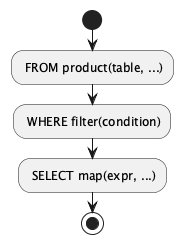
\includegraphics[height=0.81\textheight]{from_where_select.tikz}
    \end{center}

\end{frame}

\begin{frame}[fragile]
    \frametitle{SELECT in Python}

    \begin{itemize}
    \item[]
        \texttt{FROM t1, t2, ...}

        \begin{minted}[autogobble]{python}
        from_ = itertools.product(t1, t2, ...)
        \end{minted}

        \vspace{1em}
    \item[]
        \texttt{WHERE c}

        \begin{minted}[autogobble]{python}
        where = (row_tuple
            for row_tuple in from_
                if c(row_tuple))
        \end{minted}

        \vspace{1em}
    \item[]
        \texttt{SELECT ex1, ex2, ...}

        \begin{minted}[autogobble]{python}
        result = list(
            (ex1(row_tuple), ex2(row_tuple), ...)
            for row_tuple in where)
        \end{minted}

    \end{itemize}

\end{frame}

\begin{frame}
    \frametitle{Good and Bad}

    \begin{itemize}
    \item The Python code matches the SQL.

    \item A lot more syntax: \texttt{WHERE expr} becomes \texttt{(r for r in from\_ if expr)},

    \item \texttt{SELECT expr, expr, expr} is even \textbf{more} complicated-looking.
    \end{itemize}

    \vspace{1em}
    Let's look at details. All the syntax means there are a lot of places to add processing.
\end{frame}

\section{Python Implementation Patterns}

\begin{frame}[fragile]
    \frametitle{The From Clause}

    The \texttt{FROM} tables need to be iterable sequences.

    \texttt{list[dict[str, Any]]}

    \vspace{1em}
    \begin{minted}[autogobble]{python}
    from itertools import product

    from_ = product(t1, t2, t3)
    \end{minted}

    \vspace{1em}
    Yes. It's the Cartesian product.

\end{frame}

\begin{frame}[fragile]
    \frametitle{Aha!}

    \begin{alertblock}{``Gotcha!''}
    \begin{itemize}
        \item A \textit{real} database doen't do cartesian products all the time.

        \item It has fancy query algorithms and optimizations. \pause
    \end{itemize}
    \end{alertblock}

    \vspace{1em}

    ``Your nonsense is clearly unworkable in general.''
\end{frame}

\begin{frame}[fragile]
    \frametitle{Query optimization}

    \begin{itemize}
    \item Requires extended syntax to suggest query optimizations.

    \item Require someone to design the right indexes.

    \item Requires detailed statistics on key distribution.
    \end{itemize}

    \vspace{1em}

    You \textbf{can} do this query optimization in Python, also.\pause
    \vspace{1em}

    We'll get to it.
\end{frame}


\begin{frame}[fragile]
    \frametitle{The Where Condition}
    \textbf{Context:}

    \begin{minted}[autogobble]{python}
    where = (row for row in from_ if c(row))
    \end{minted}

    Or.

    \begin{minted}[autogobble]{python}
    where = filter(c, from_)
    \end{minted}


    \vspace{1em}
    \begin{minted}[autogobble]{python}
    def c(row: tuple[dict[str, Any], ...]) -> bool:
        t1, t2, t3 = row
        return (
            t1['rowid'] == t2['foreign_key']
            and t2['some_key'] == t3['whatever']
        )
    \end{minted}


\end{frame}

\begin{frame}[fragile]
    \frametitle{The Select Clause}
    \textbf{Context:}

    \begin{minted}[autogobble]{python}
    result = list(
        (ex1(row_tuple), ex2(row_tuple), ...)
        for row_tuple in where)
    \end{minted}

    Or.

    \begin{minted}[autogobble]{python}
    result = map(row_builder, where)
    \end{minted}

    \vspace{1em}
    \begin{minted}[autogobble]{python}
    def e1(row: tuple[dict[str, Any], ...]) -> Any:
        t1, t2, t3 = row
        if t1['value'] % 2 == 0:
            return t1['value'] // 2
        else:
            return t1['value'] * 3 + 1
    \end{minted}

\end{frame}

\begin{frame}
    Okay, \texttt{From}, \texttt{Where}, and \texttt{Select} clauses not awful. \pause

    \vspace{1em}

    The \texttt{From} clause needs work.
\end{frame}

\section{About Those Join Algorithms}
\begin{frame}
    \frametitle{The Cartesian Product Problem}

    Databases do ``cart-prod'' joins all the time.

    \vspace{1em}
    Very small tables are easier to fetch from disk into cache without wasting time on the additional index read.

    \vspace{1em}
    Two common alternative algorithms:
    \begin{itemize}
        \item Sort-Merge Join
        \item Lookup Join
    \end{itemize}
\end{frame}

\begin{frame}
    \frametitle{Sort-Merge Join}

    For very large tables.

    \begin{enumerate}
    \item Sort each table into a consistent order by the join key for that table.

    \item Create row tuples for matching rows from each sorted table.
    \end{enumerate}

    \vspace{1em}

    A variation on this can do any of the outer join algorithms.

    \vspace{1em}

    See \texttt{\underline{https://toolz.readthedocs.io}}; they offer \texttt{merge\_sorted()}

\end{frame}


\begin{frame}[fragile]
    \frametitle{Lookup Join}

    Greate for many small tables and one big table.

    The ``Star Schema'' design pattern.

    \vspace{1em}
    Transform each small table into a Python dictionary.

    Then, this:
    \begin{minted}[autogobble]{python}
    from_ = (
        (r, small_1[r['key_1']], small_2[r['key_2']])
        for r in big_table
    )
    \end{minted}
\end{frame}

\begin{frame}
    Okay.
    \vspace{1em}

    Fine.
    \vspace{1em}

    The \texttt{From}, \texttt{Where}, and \texttt{Select} clauses have really fast pure-Python implementations.
    \vspace{1em}

    What about \texttt{Group by} and \texttt{Having}?  \pause

    They can't be simple.
\end{frame}

\section{Group By and Having --- The Good Stuff}
\begin{frame}
    \frametitle{Group By Clause(s)}

    The \textbf{Group By} process involves two separate things.
    \begin{itemize}
        \item The expressions (and column names) in the \texttt{GROUP BY} clause.

        \vspace{0.8em}
        These expressions define a kind of \texttt{reduce()} function to build the groups.

        \vspace{1em}
        \item The Aggregate Functions in the \texttt{SELECT} clause then get applied to each group's subset of rows.
    \end{itemize}

    \vspace{1em}

    Syntax Oddity: Aggregates written in the \texttt{SELECT} clause.
    Some in the \texttt{HAVING} clause.

\end{frame}

\begin{frame}
    \frametitle{Group By Implementation}

    \begin{enumerate}
        \item Parition into groups, \texttt{defaultdict(list)}.

        For each row:
        \begin{enumerate}
            \item Create keys
            \item Append row to groups
        \end{enumerate}

        \item For each group:
        \begin{enumerate}
            \item Evaluate all the aggregate functions.
        \end{enumerate}

    \end{enumerate}

    \vspace{1em}
    This builds a new table from the keys and aggregate functions for each group.
\end{frame}

\begin{frame}[fragile]
    \frametitle{Group By Implementation}

    \begin{minted}[autogobble]{python}
    from collections import defaultdict
    from operator import itemgetter
    # Partition
    groups = defaultdict(list)
    for row_tuple in where:
        key = (k_1(row_tuple), k_2(row_tuple), ...)
        groups[key].append(row_tuple)
    # Aggregate
    group_by = []
    for key, group in groups:
        agg_1 = some_function(group)
        agg_2 = mean(row['value'] for row in group)
        agg_3 = sum(map(itemgetter('name'), group))
        group_by.append((key, agg_1, agg_2, agg_3))
    \end{minted}

\end{frame}

\begin{frame}
    \frametitle{Having Clause}

    The \texttt{Having} process is (nearly) the same as the \texttt{Where} process.

    It's an expression to filter the groups.

    \vspace{1em}

    SQL syntax uses aggregate functions in the \texttt{Having} clause.

    \begin{itemize}
        \item These are yet more group-by aggregates.

        \item The result values are only used for filtering.
    \end{itemize}

\end{frame}

\section{Conclusion}
\begin{frame}
    \frametitle{Conclusion}

    \begin{itemize}
        \item SQL is helpful to summarize a desired result.
        \item SQL can be overused.
        \item A database is a lot of overhead. Avoid it.
    \end{itemize}
    \vspace{1em}
    Think of SQL as a design language.\pause

    Not an implementation choice.
\end{frame}

\begin{frame}
    \frametitle{SQL}

    \begin{itemize}
        \item SQL describes a pipeline of steps
        \[
            \textrm{From} \rightarrow \textrm{Where} \rightarrow \textrm{Select} \rightarrow \textrm{Group By} \rightarrow \textrm{Having}
        \]

        \item Or. As nested functions
        \[
            H\Biggl(G_A \biggl (G_P \biggl( S \Bigl(W \bigl( F(t_1, t_2, ...) \bigr) \Bigr) \biggr)\biggr)\Biggr)
        \]

        \end{itemize}

        Nested functions seem confusing.

\end{frame}

\begin{frame}[fragile]
    \frametitle{SQL to Python}
    In Python, \texttt{Select} is a stack of generator expressions

    \begin{minted}[autogobble,fontsize=\scriptsize]{python}
        from_ = itertools.product(...)
        where = filter(condition, from_)
        select = map(row_builder, where)
        groups = group_reduce(select)
        aggregates = map(agg_row_builder, groups)
        result = filter(having_condition, aggregates)
    \end{minted}

    Most steps are lazy and don't compute big intermediate results. \pause

    The \texttt{group\_reduce()} function does compute a big result.

\end{frame}

\begin{frame}
    \frametitle{Call to Action}
    Stop using SQL as a data transformation tool.

    \vspace{1em}
    Continue using SQL as a design aid.
\end{frame}

\begin{frame}
    \frametitle{More Information}

    \begin{itemize}
        \item \textit{Unlearning SQL} (Available from Amazon and Lulu) \vspace{1em}
        \item \texttt{\underline{https://github.com/slott56/functional-SQL}} \vspace{1em}
        \item \texttt{\underline{https://fosstodon.org/@slott56}}
    \end{itemize}
\end{frame}

\end{document}
